\documentclass[10pt,a4paper,twoside,openright]{memoir}
\usepackage[utf8]{inputenc}
\usepackage[english]{babel}

% ----- pgfplots -----
\usepackage{femtikz} % pgfplots, tikz, graphicx
%\tikzexternalize

% ----- formatting -----
\usepackage{titling}
\usepackage{fancyhdr}
\usepackage{enumitem} % resume
%\usepackage{booktabs}
\OnehalfSpacing % memoir
\nouppercaseheads % memoir
%\setsecnumdepth{subsection} % memoir
%\maxtocdepth{subsection} % memoir
\newcommand{\h}{\textit{h}}
\newcommand{\p}{\textit{p}}
\newcommand{\hp}{\textit{hp}}

\newcommand{\dealii}{\texttt{deal.II}}
\newcommand{\pforest}{\texttt{p4est}}
\newcommand{\petsc}{\texttt{PETSc}}
\newcommand{\trilinos}{\texttt{Trilinos}}
\newcommand{\epetra}{\texttt{Epetra}}
\newcommand{\aztecoo}{\texttt{AztecOO}}
\newcommand{\ml}{\texttt{ML}}
\newcommand{\xsdk}{\texttt{xSDK}}

\newcommand{\opencascade}{\texttt{OpenCASCADE}}
\newcommand{\opensalome}{\texttt{OpenSALOME}}
\newcommand{\fftw}{\texttt{FFTW}}
\newcommand{\mofem}{\texttt{MoFEM}}
\newcommand{\phg}{\texttt{PHG}}
\newcommand{\phaml}{\texttt{PHAML}}


% ----- miscellaneous -----
\usepackage{doi} %necessary?

% ----- work in progress -----
\usepackage{todonotes}
\usepackage{blindtext}
\usepackage{showframe}

% ----- math -----
\usepackage{amsmath,amsfonts,amssymb}
\usepackage{isomath} % \vectorsym, \matrixsym, \tensorsym
\usepackage{bbold}
\DeclareMathOperator{\Froude}{Fr}
\DeclareMathOperator{\Mach}{Ma}
\DeclareMathOperator{\Prandtl}{Pr}
\DeclareMathOperator{\Reynolds}{Re}
\DeclareMathOperator{\Strouhal}{St}

\newcommand{\differential}[1]{\ensuremath{\mathop{}\!\mathrm{d}#1}}
\renewcommand{\vec}[1]{\ensuremath{\vectorsym{#1}}}
\newcommand{\mat}[1]{\ensuremath{\matrixsym{#1}}}
\newcommand{\ten}[1]{\ensuremath{\tensorsym{#1}}}

\newcommand{\source}[1]{\ensuremath{\dot{#1}'''}}

% ----- bibliography -----
\usepackage[backend=biber, style=authoryear]{biblatex}
\DefineBibliographyStrings{english}{citedas = {hereafter}}
\bibliography{misc/bibliography.bib}

% replace 'note' by 'shorthand' for: MPI, OpenMP, CUDA, TBB, OpenACC
\immediate\write18{sh misc/convert-shorthand.sh misc/bibliography.bib}

% print url and urldate only if there is no doi
\DeclareSourcemap{
  \maps[datatype=bibtex]{
    \map{
      \step[fieldsource=doi,final]
      \step[fieldset=url,null]
      \step[fieldset=urldate,null]
    }  
  }
}

% ----- glossary -----
\usepackage[automake]{glossaries-extra}
\makeglossaries
\newabbreviation{cpu}{CPU}{central processing unit}
\newabbreviation{gpu}{GPU}{graphics processing unit}

\newabbreviation{api}{API}{application programming interface}
\newabbreviation{cuda}{CUDA}{Compute Unified Device Architecture}
\newabbreviation{mpi}{MPI}{Message Passing Interface}
\newabbreviation{openacc}{OpenACC}{Open Accelerators}
\newabbreviation{openmp}{OpenMP}{Open Multi-Processing}
\newabbreviation{tbb}{TBB}{Threading Building Blocks}

\newabbreviation{cfd}{CFD}{computational fluid dynamics}

\newabbreviation{hpc}{HPC}{high-performance computing}

\newabbreviation[plural={FDM}, \glsshortpluralkey={FDM}]{fdm}{FDM}{finite difference method}
\newabbreviation[plural={FVM}, \glsshortpluralkey={FVM}]{fvm}{FVM}{finite volume method}
\newabbreviation[plural={FEM}, \glsshortpluralkey={FEM}]{fem}{FEM}{finite element method}
\newabbreviation{fft}{FFT}{fast Fourier transformation}
\newabbreviation{lbm}{LBM}{lattice Boltzmann method}

\newabbreviation[longplural={degrees of freedom}]{dof}{DoF}{degree of freedom}

\newabbreviation{amr}{AMR}{adaptive mesh refinement}
\newabbreviation{simd}{SIMD}{single instruction, multiple data}

\newabbreviation{cg}{CG}{continuous Galerkin}
\newabbreviation{dg}{DG}{discontinuous Galerkin}

\newabbreviation{amg}{AMG}{algebraic multigrid}
\newabbreviation{gmg}{GMG}{geometric multigrid}

\newabbreviation{xsdk}{\xsdk{}}{extreme-scale scientific software development kit}



% --- document information ---
\author{Marc Fehling}
\title{Algorithms for massively parallel hp--adaptive finite element methods}
\date{31. April 2020}



\begin{document}
  \begin{titlingpage}
    \begin{center}
      \vspace*{\fill}
      \includegraphics[width=.75\textwidth]{logos/BUW_Logo-schwarz.eps}\bigskip
      \vspace*{\fill}\vspace*{\fill}\par
      {\Huge \thetitle\bigskip\par}
      {\Huge \theauthor\bigskip\par}
      {\LARGE \thedate\bigskip\bigskip\par}
    \end{center}
    {\large Perfect Publishing\hspace*{\fill}Forward by Fabulous Freddy\smallskip\\
    The World\hspace*{\fill}Author of \emph{Kayaking with dragons}}
  \end{titlingpage}
  
  
  
  \frontmatter
  
  \abstractintoc
  \begin{abstract}
    Abstract.
  \end{abstract}
  \clearpage
  
  % Approval page
  
  \begin{KeepFromToc} % memoir
    \tableofcontents
  \end{KeepFromToc}
  \clearpage
  
  % Dedication
  
  % Acknowledgements
  
  \listoftables
  \clearpage
  
  \listoffigures
  \clearpage
  
  \printglossary[type=\acronymtype, title={List of Abbreviations}]
  
  % Other lists
  
  % Preface
  
  
  
  \mainmatter
  
  \chapter{Introduction}
\label{ch:introduction}
\glsresetall

%\todo{Introduction:}
%\begin{itemize}
%  \item Need for new computational methods (adaptive)
%  \item Statistics on usage of FDS? (literatur aus bennis diss?)
%  
%  \item Latest catastrophes: tower, Düsseldorf
%  \item ... help to .. catastrophes by giving hints on placements of safety measures.
%\end{itemize}

% introduction

For the analysis of most problems in science and engineering, mathematical modeling is required to capture underlying correlations and apply findings to related variations. With rising complexity of the model, an analytical solution of a problem so described is less likely to exist, and can only be acquired via approximation with numerical methods. Computers are used today to solve these kinds of problems numerically, but depending on the complexity of the problem and the computer hardware used, such analyses can have exceptionally long execution times.

An intelligent distribution of the computing resources, which due to the dynamics of a simulation does not have to be done \textit{a priori} but progressively, can be used to reduce the computing time (\textit{strong scaling}), and to provide more accurate results in the same execution time (\textit{weak scaling}). This is possible both physically by workload distribution to several processors
% exploiting the hardware structure
and logically by
an adaptive resolution of the simulation%
% allocating resources to critical operations
, in each case based on the current state of the simulation.
Recent advancements in computer technology allows us to solve problems with billions of unknowns. However, raw computing power does not mean we can use it without further ado. Only the combination with algorithms that use all available resources efficiently and scale with the problem size offers a massive potential to reduce execution times.
%The keys to efficiency are algorithms that exploit the hardware structure and focus resources on critical operations.
The goal of this dissertation is the provision of such new, efficient algorithms.

% algorithms on hardware level

Applications can be optimized for the hardware structure up to the instruction level, for example using \gls{simd} instructions combined with vectorization, and by avoiding bottlenecks caused by memory and network bandwidth.
Furthermore, modern multi-core and multi-processor systems require parallelization to make hardware threads and processes cooperate with each other, respectively. %, which highly depends on hardware architecture.
%on which we will focus in this dissertation.
%The choice of parallelization highly depends on hardware architecture, and are a requirement for large-scale supercomputers with distributed memory access.
Depending on the hardware architecture, many different \glspl{api} have been developed over the last decades which allow developers to take opportunity of unified interfaces.
For machines with shared memory access like modern desktop workstations, independent computing tasks can be distributed among all hardware threads subjecting to a work stealing policy, for which \gls{openmp}\textsuperscript{\textregistered} \textcite{openmp50} and Intel\textsuperscript{\textregistered} \gls{tbb} \textcite{tbb2018} are the most prominent approaches.
On large-scale supercomputers, processes are spread out on multiple computing nodes with independent memory segments connected via network. To enable them to cooperate, data needs to be exchanged between all participating nodes. For communication between processes, the \gls{mpi} \textcite{mpi31} has become a standard. A hybrid combination of both techniques for shared and distributed memory is possible.
%If architecture is distributed on nodes and thus have distributed memory access, the \gls{mpi} \textcite{mpi31} will be used.
Recently, streaming multiprocessor architectures on \glspl{gpu} have become of more and more interest for scientific applications, which offer lots of theoretical throughput, but are strongly limited in flexibility. \gls{openacc}\textsuperscript{\textregistered} \textcite{openacc27} and Nvidia\textsuperscript{\textregistered} \gls{cuda}\textsuperscript{\textregistered} \textcite{cuda10} provide interfaces for the scientific use of \glspl{gpu}.

% methods for spatial discretization

Numerical methods require the discretization of the continuous space which will be divided into smaller entities that couple with neighboring ones. A large variety of these methods exist, of which we briefly describe the most commonly used ones.
With \glspl{fdm}, differential operators are evaluated as difference quotients on a finite number of grid points. %Those are easy to implement, but inflexible
The idea of \glspl{fvm} is the preservation of conserved quantities on small volumes by applying the Gauss-Ostrogradski theorem, which results in balancing volumetric averages with fluxes on interfaces of neighboring volumes.
%With the \gls{fvm}, conserved quantities are preserved on small volumes applying the Gauss-Ostrogradsky theorem, resulting in balancing volumetric averages and fluxes on interfaces.
In \glspl{fem}, we specify a function space of piecewise polynomials in which we find the function 
%is supposed to be part of, and find the representation
that minimizes the residual of the investigated problem.
%\gls{fem} contains \gls{fvm} intrinsically if you consider piecewise constant functions.

% algorithms for adaptation

In addition to optimizing numerical methods to the hardware, we can also adjust the numerical discretization to the local complexity of the investigated problem by adapting its resolution.
%we can also on a logical level by focusing computational resources on critical sections of the investigated problem.
%On the other hand, focus computational ressources on critical sections of the domain, which are problem dependet and  These sections . adaptive
This does not only assure the full utilization of all available resources, but also their efficient usage.
%The key to use those ausnutzen fully are efficient algorithms that either fit to the hardware or distribute resources on computing intensive operations.
%A combinatation of both hardware and .. software driven algorithms can be supplied. However, their combination is not trivial.
%Adaptive methods assign resolution of the problem on interesting parts of the domain.
%A common approach is adapting the numerical discretization to the specifics of the investigated problem.
With \gls{amr}, or \h-adaptive refinement, the spatial resolution of our discretization will be locally assigned, resulting in entities with different sizes $h$. While \gls{fdm} requires a regular topology for \gls{amr}, it is applicable on \gls{fvm} and \gls{fem} without major restrictions. In addition, \gls{fem} offers the unique capability for \p-adaptation, in which the polynomial degree of the basis functions is locally set. The combination of both is possible, resulting in \hp-adaptive methods.
%, which are the focus of this dissertation.

% universal application of these methods

The presented algorithms can be applied on various problems involving partial differential equations from mathematics, nature, and engineering. They have already been extensively used for e.g.\@ structural mechanics, heat transfer, wave propagation, electrostatics, and fluid dynamics to name just a few.
In engineering practice, these methods form the basis for simulations on objects, for instance to investigate their stress and wear behavior and to generate their flow profile. Corresponding model experiments are complex and expensive, so computer simulations offer an alternative.
A concrete application example describes the simulation of smoke spread in buildings.
On basis of their results, fire safety engineers are able to optimize smoke extraction systems and evacuation routes to increase the safety of civilians in the event of a fire outbreak.
In general, fires remain spatially localized even after their ignition phase, so the dynamic allocation of both resolution and computational resources is highly favorable in this scenario.
Their simulation on large scale buildings or connected facilities like underground tunnel systems as investigated in the ORPHEUS project \parencite{arnold2017}, yield an incredible amount of workload.
%a use of adaptive methods . and the combination with parallelization on large-scale buildings, or even large connected facilities like underground stations as investigated in the \texttt{ORPHEUS} project, yield a lot of complexity and thus a lot of workload.

%Further, the combination of an efficient use of computational ressource via parallelization as well as an intelligent assignment of these ressource on crucial areas of the problem via adaptation is incredibly important.

Thus, the combination of parallelization and adaptive methods is necessary to perform simulations on an economically acceptable time scale. However, their implementation is very difficult with lots of technical finesses to consider.
%The combination of both parallelization with adaptative methods is necessary is highly favorable, but very difficult to implement with lots of technical finesses to consider.
%Both methods require lots of technical finesses to make them availble. as well as mathematical ... .
%Although there are many software solutions that offer parallel \h-adaptive methods, only a few offer \hp-adaptive methods and even less combine it with parallelization.
Many software solutions for parallel \h-adaptive methods exist, however their \hp-adaptive equivalents are rarely realized because of their complexity.
In this dissertation, we will focus on \hp-adaptive \gls{fem} with their exceptional error convergence properties \parencite{guo1986,babuska1996}, and provide their parallelization for distributed memory systems.
%This thesis presents the combination of both parallelization on distributed hardware architecture, and hp-adaptive methods.

% existing software solutions

%\textcite{shahbazi2007}

In the past, several algorithms for parallel \hp-adaptive \gls{fem} have been developed, but they always stayed in the context of \gls{dg} methods which allow solutions to be discontinuous across cell interfaces. For example for Navier-Stokes problems, \textcites{paszynski2006}{chalmers2019} presented methods for distributed memory architectures, while \textcites{paszynski2011}{jomo2017} demonstrated methods for shared memory machines. A general approach which also works with \gls{cg} methods poses additional implementation challenges that are pointed out in the course of this dissertation. %and has not been published yet.

%\textcite{paszynski2006}
% demkovisz par

Due to their complexity, \hp-adaptive methods have always stayed in an experimental stage and have never been prepared to be easily applied by a broader academic audience, especially in combination with parallelization.
Though, there are several open-source libraries available to the public that provide the bare functionality for \hp-adaptive \gls{fem} on distributed memory architectures using the \gls{mpi} protocol, such as the libraries \phaml{} \parencite{mitchell2002,phaml1200}, \phg{} \parencite{zhanglin-bo2019,phg094}, and \mofem{} \parencite{kaczmarczyk2020,mofem090}. However, even here the application of these features is not immediately accessible to the end user. We are not aware of any commercial tools capable of this feature.

% par3dhp - not publicly available
% hermes - only openmp parallelization

% deal.II

%Further, although parallel \hp-adaptive \glspl{fem} have been presented thoroughly, there is no systematic description on how to realize them yet as a software application. There are publications that highlight all necessary data structures and algorithms parallelization \parencite{bangerth2012} (parallel paper) and \hp-adaptive methods \parencite{bangerth2009}.

Furthermore, although applications of parallel \hp-adaptive \glspl{fem} have been presented thoroughly, there is no systematic description on how to realize them yet as a software implementation.
Algorithms and data structures have already been presented in detail for parallel \h-adaptive \gls{fem} by \textcite{bangerth2012} and sequential \hp-adaptive \gls{fem} by \textcite{bangerth2009}.
%However, the combination of both elaborations is not trivial and has not yet been carried out.
The goal of this dissertation is to provide the combination of both algorithms highlighting difficulties to combine both parallelization with \hp-adaptive methods. This dissertation is not meant to be an in-depth guide for the creation of \gls{fem} software. We would rather like to emphasize on the basic ideas for parallel \hp-adaptive \gls{fem} and point out programming challenges. We will provide an example implementation in the \dealii{} library \parencite{bangerth2007, dealii920pre}, so that the reader is able to either embed our findings into their own \gls{fem} code or use the \dealii{} implementation right away.

\dealii{} is an open-source software library for the creation of general purpose \gls{fem} codes.
%It offers lots of additional features for \gls{fem} that go beyond usual
%With it, users can easily generate their own application for scientific research on basis of the expertise of their developers.
It is part of the \gls{xsdk} \parencite{bartlett2017,xsdk050},
%and builds upon interfaces to other libraries providing .
which combines efforts of many research software engineers to make their expertise in optimized \gls{hpc} available and provides them to the public as a whole.
%and combine it with to all packages in this kit
%from which all packages in this kit profit.
%share their own expertise and benefit from others
%It is a joint effort to provide a set of tools for exascale computing.
%relying on the expertise of other developers and their
%and offers lots of features
In this context of sharing knowledge, \dealii{} profits from parallel linear algebra provided by the open-source libraries \trilinos{} \parencite{heroux2005,trilinos12181} and \petsc{} \parencite{balay2019,petsc3124}, and utilizes their implementation via designated interfaces.
%In the \dealii{} library, we rely on third party libraries. Parallel linear algebra by \trilinos{} \parencite{heroux2005,trilinos12181} and \petsc{} \parencite{balay2019,petsc3124}.

Furthermore, \dealii{} does not provide the hierarchic generation of \h-adaptive meshes and their partitioning on multiple processes of distributed memory architectures itself, but relies on the implementation of the open-source library \pforest{} \parencite{burstedde2011,p4est22}. In this regard, \pforest{} is used as an `oracle': Operations that manipulate the mesh and its partitioning happen on a distributed structure provided by \pforest{}, and will be recreated only on the locally owned sections of the \dealii{} mesh
%and data structures
on every process with a set of queries to the master mesh.
%Every cell related data is thus stored in both libs in the very same way. They both use Z-order or Molten-schemes to iterate over cells. (sth like that?)

Since the ideas of this dissertation will be realized in \dealii{}, we capitalize on their hierarchic quadtree and octree structures with corresponding quadrilateral and hexahedral cells in two and three dimensions, which are arranged by means of a Z-order or Morton space-filling curve.
%The combination of \dealii{} and \pforest{} poses restrictions based on decisions made during their development process, for example the specialization on hierarchic quadtree and octree structures with corresponding quadrilateral and hexahedral cells in two and three dimensions, which will be arranged by means of a Z-order or Morton space-filling curve.
%Although the combination of \dealii{} and \pforest{} relies on quadrilateral and hexahedral cells in two and three dimensions for which they use a Z-order or Morton scheme
However, the presented ideas for algorithms and data structures in this dissertation are not restricted to these specifications.

% thesis outline

%Algorithms and data structures have already been presented for parallel \h-adaptive \gls{fem} by \textcite{bangerth2012} and sequential \hp-adaptive \gls{fem} by \textcite{bangerth2009}. However, the combination of both elaborations is not trivial.

In this dissertation, we present all enhancements necessary to supply parallel \hp-adaptive methods for algorithms and data structures that are already capable of parallel \h-adaptive and sequential \hp-adaptive \gls{fem}. In Ch.~\ref{ch:parallel} we present the necessary details for static meshes, i.e.\@ meshes with fixed resolution and assignment of finite elements from beginning to end of a simulation. Ch.~\ref{ch:dynamic} deals with all necessities of dynamic \hp-adaptive methods, and presents algorithms to automatically determine regions to adapt. We apply the presented methods on a simple numerical example in Ch.~\ref{ch:results} to show the benefits of \hp-adaptive methods and the scalability on the JURECA supercomputer \parencite{krause2016,jureca}.

Some of the algorithms presented in this dissertation have already been published in the current release of the \dealii{} library \parencite{arndt2019} and their entirety will be made available completely with the upcoming release. All numerical examples in this dissertation have been performed using a certain version of the library published on a public fork \textcite{finaldissertation} of the corresponding \dealii{} repository \textcite{dealii920pre}.

  \chapter{Massively parallel \hp-adaptive \glsfmtlongpl{fem}}
\label{ch:parallel}
\glsresetall

Any kind of numerical method requires thorough thought on designing suitable algorithms and data structures with respect to correctness, robustness and performance. In general, the ideas behind implementations of these methods are similar and can be generalized.
%, especially when they are based on the same numerical method.
This is also the case for additional enhancements that improve basic realizations. In case of the \gls{fem} such features are, for example, parallelisation, adaptive methods, continuous or discontinuous Galerkin methods, and the support for complex geometries.

In this chapter, we will present algorithms and data structures for parallel, \hp-adaptive \glsfmtlongpl{fem}. Generalized thoughts on each of the two aspects have already been presented: \textcite{bangerth2009} developed a general implementation for \hp-adaptive \gls{fem} software; and a generalized distributed computing approach of the \glsfmtlong{fem} has been introduced by \textcite{bangerth2012}. However, the consolidation of both features is not trivial. We will elaborate on the trickiest facets in the following sections, after providing a brief introduction to \gls{fem} and the parallelisation approach we will follow.

Thus chapter should be understood as an enhancement of the two aforementioned contributions and bases on large parts on it. We recommend a previous reading of both articles.


\subsubsection{Basics of the \glsfmtlong{fem}}

The basic idea of the \glsfmtlong{fem} conforms to the specification of a function space and finding a solution to the investigated problem in it. To be more precise, we pick a suitable set of basis functions for which the solution is a linear combination. Its coefficients are called unknowns or \glspl{dof}, since their values are determined after solving the problem.

In general, \gls{fem} requires a subdivision of the domain into smaller cells, typically into triangles or quadrilaterals in two and tetrahedra or hexahedra in three dimensions. All these cells are mappings of a reference cell, to which we assign a set of shape functions with corresponding support points.
%Those functions are designed to have the value one on exactly one support point and the value zero on all others.
The composition of reference cell, shape functions and support points is defined as a finite element.

The collection of all cells with their corresponding finite elements assigned form the aforementioned function space. In the global mesh, each support point for each finite element will be uniquely identified with a \gls{dof} on each cell. Consulting the weak formulation of the investigated problem, we are then able to formulate and solve the corresponding system of linear equations.

\todo{add some equations and math symbols}
$u_h(\vec{x}) = \sum_{j=0}^{N-1} U_j \varphi_j(\vec{x})$
% $u_h \in V_h$

This is just a brief introduction to \gls{fem} in order to provide the fundamentals for this chapter and to specify the nomenclature used. More details on this topic can be found in common literature \parencite[e.g.][]{girault1986, elman2014, kuzmin2015} \todo{add more literature?}. Especially \textcite{brenner2008} provided a more rigorous and mathematically sound definition on finite elements.


\subsubsection{Parallelization approach for adaptive meshes}

For distributed computing.

This involves a hierarchy

However, to stay flexible during 

This is just a brief outline of all the requirements that \textcite{bangerth2012} worked out, which is crucial for the upcoming section.


\section{Enumeration of \glsfmtlongpl{dof}}
\label{sec:enumeration}

Text.
\section{Data transfer}
\label{sec:transfer}

Text.

Without \p-adaptivity, the number of \glspl{dof} or rather the amount of data to store per cell does not differ. Thus, we know how much data to send or receive on each cell. This is no longer the case with \p-adaptivity.
\section{Load balancing}
\label{sec:balancing}

The efficient use of all computational resources requires a uniform distribution of all workload among them. There are many factors that determine the workload in a \gls{fem} application, above all the preparation of data structures, the assembly of both the matrix and right hand side of the linear equation system, and the choice of the type of its solver.

In most \h-adaptive applications, cells are similar and correspond to the same workload. Thus, we can simply balance the number of cells on all processes. However with \hp-adaptive application, this is no longer the case due to the diversity of finite elements. %Here, the workload varies with the number of \glspl{dof} on each cell. (and the quadrature)
In this case, since the domain is partitioned on the basis of cells, we need to assign a corresponding weight to every cell that determines its individual workload and balance the cumulated weights among all processes.

The workload of each cell depends on its assigned finite element and quadrature formula, and correlates to the number of \glspl{dof} and quadrature points, among other quantifiable values that depend on the individual problem. For example, Lagrangian elements of different order as depicted in Fig.~\ref{fig:lagrange} each have a distinct number of \glspl{dof} assigned.

%For example, consider Lagrangian elements of different polynomial degrees with different number of \glspl{dof} depicted in Fig.~\ref{fig:lagrange} require a different workload, mainly consumed by matrix assembly and the solution process.

%and can be quantified
%We expect a correlation of every cell's individual workload with the assigned number of \glspl{dof} and number of quadrature point of the assigned formula, among others quantifiable values.

%Ideally, we want to balance the workload. We will thus perform weighting.

%and balance the cumulated sum of cells to be equal on all processes. We can do that with a prefix sum.

For the purpose of load balancing, \textcite[Sec.~3.3]{burstedde2011} provided an algorithm for weighted partitioning and enhanced \pforest{} \textcite{p4est22} with a corresponding implementation, from which we take advantage in \dealii{}. Omitting details about the communication between processes, we will briefly outline its basic idea: On a distributed mesh, calculate the prefix sum of cell weights in the global scope, determine the partition boundaries with a binary search, and transfer cells to their new owning processes if necessary.

%The partitioning algorithm of \pforest{}

%\pforest{} offers such a weighting mechanism. The basic idea behind it is, that we calculate the cumulated sum of cells with a prefix sum, and assigning the correpsonding partition to our process with a binary search.

%We rely on the implementation of \textcite{burstedde2018} in \pforest{} \textcite{p4est22}. The basic idea of this algorithm is to form a cumulated of all cell weights with an \texttt{MPI\_Exscan} call, and then each process will find its balanced range of cells with binary searches.

In the context of \hp-adaptive \gls{fem} applications, we identify the assembly of the linear equation system and its solution as the most expensive tasks, and correlate their individual contribution to the workload on each cell with the number of \glspl{dof} from the assigned finite element.
%As a first indicator for the workload, we make the number of \glspl{dof} responsible.
The workload of efficient solvers scales with the number of \glspl{dof} $\mathcal{O}\left(n_\text{dofs}\right)$, while we suppose that the workload of the assembly will be of order $\mathcal{O}\left(n_\text{dofs}^2\right)$ since we fill quadratic matrices.

We expect that the actual workload of an \hp-adaptive \gls{fem} application will actually scale with an order somewhere in between the two, i.e.\@ $\mathcal{O}\left(n_\text{dofs}^c\right)$ with a constant exponent $c \in [1,2]$. We use this strategy for investigations in this dissertation in which we also determine a suitable exponent $c$.

Alternatively, weighting each cell with a factor of $(a \, n_\text{dofs}^2 + b \, n_\text{dofs})$ appears conceivable, for which the partitioning results depend on the ratio of both constants $a$ and $b$.

%We will assign a weight $n_\text{dofs}^i$ to every cell, % and balance the cumulated sum of cells to be equal on all processes. We can do that with a prefix sum.

A reliable measure of weights is tied to the type of problem and the choice of the solver. With the presented approach, we still have to specify a suitable weight manually. It is part of future work to supply a heuristic from which we will determine suitable weights automatically. %, depending on the type of problem and the choice of the solver.
  \chapter{Dynamic \hp-adaptive \glsfmtlongpl{fem}}
\label{ch:dynamic}

Text.



\section{Realization of \hp-adaptation}
\label{sec:adaptation}

For \hp{}-adaptive methods we need to find ways to prescribe which cells are subject to which kind of adaptation. This grants awareness on how the mesh will change if adaptation is executed.

To indicate that adaptation is about to happen, we introduce general flags for refinement and coarsening, respectively. We are left to distinguish between \h- and \p-adaptation. To do this, we specify so called \textit{future finite element} indices that determine the finite element that will be associated to that particular cell after adaptation has been performed. If such a future finite element is defined on marked cells, \p-adaptation will be performed, while cells will be \h-adapted if none is specified. This approach offers full flexibility to let either users decide manually how to adapt, but also provides a sufficient interface for an automatic specification of these mesh attributes.

To determine the extent to which cells change during the adaptation process, the affected cell properties have to be hierarchically ordered. While for \h-adaptive methods, a grid hierarchy naturally evolves from the underlying tree or forest data structure, this is not necessarily the case for \p-adaptation. Here, a hierarchy needs to be provided for the collection of finite elements, so that we can assign superior and subordinate elements in case of \p-refinement or \p-coarsening, respectively. For example, we arrange Lagrangian finite elements by their polynomial degree in ascending order with the largest degree on the highest level.

Executing \h-adaptation on a \p-adapted mesh reveals another challenge. We need to find a suitable finite element on cells that will be \h-adapted. During \h-refinement, we can easily choose the finite element from the parent cell for all of its children, but for \p-coarsening, the choice is not trivial. From all cells that are going to be \h-coarsened, we pick the one finite element for the parent cell from those assigned to its children that encapsulates all of them. With simultaneous \h- and \p-adaptation, future finite elements will be considered instead of the active one. This conforms to the finite element domination logic that has been introduced by \textcite{bangerth2009} and is described in Sec.~\ref{sec:prerequisities}. An example on how finite elements are distributed during \hp-adaptation is shown in Fig.~\ref{fig:adaptation}.

\begin{figure}
\begin{subfigure}{.5\textwidth}
  \centering
  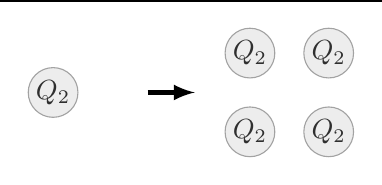
\begin{tikzpicture}[>=latex]
\def\Length{1}
\def\Radius{0.07}

% pre refinement
\LagrangeCell{0}{0}{2*\Length}{\Radius}{2}
  {{,,,,,,,,}};
\node[circle, draw=gray, fill=gray!20, inner sep=1pt, opacity=0.7, text opacity=0.8] at (\Length,\Length) {$Q_2$};

% arrow
\draw[->,ultra thick] (2.2*\Length,\Length) -- (2.8*\Length,\Length);

% post refinement
\LagrangeCell{3*\Length}{0}{\Length}{\Radius}{2}
  {{,,,,,,,,}};
\node[circle, draw=gray, fill=gray!20, inner sep=1pt, opacity=0.7, text opacity=0.8] at (3.5*\Length,0.5*\Length) {$Q_2$};

\LagrangeCell{4*\Length}{0}{\Length}{\Radius}{2}
  {{,,,,,,,,}};
\node[circle, draw=gray, fill=gray!20, inner sep=1pt, opacity=0.7, text opacity=0.8] at (4.5*\Length,0.5*\Length) {$Q_2$};

\LagrangeCell{3*\Length}{\Length}{\Length}{\Radius}{2}
  {{,,,,,,,,}};
\node[circle, draw=gray, fill=gray!20, inner sep=1pt, opacity=0.7, text opacity=0.8] at (3.5*\Length,1.5*\Length) {$Q_2$};

\LagrangeCell{4*\Length}{\Length}{\Length}{\Radius}{2}
  {{,,,,,,,,}};
\node[circle, draw=gray, fill=gray!20, inner sep=1pt, opacity=0.7, text opacity=0.8] at (4.5*\Length,1.5*\Length) {$Q_2$};
\end{tikzpicture}
  \caption{\hp-refinement.}
\end{subfigure}
\begin{subfigure}{.5\textwidth}
  \centering
  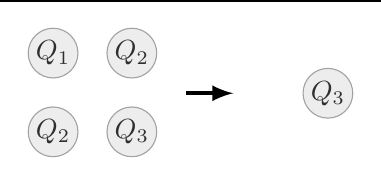
\begin{tikzpicture}[>=latex]
\def\Length{1}
\def\Radius{0.07}

% pre coarsening
\LagrangeCell{0}{0}{\Length}{\Radius}{2}
  {{,,,,,,,,}};
\node[circle, draw=gray, fill=gray!20, inner sep=1pt, opacity=0.7, text opacity=0.8] at (0.5\Length,0.5\Length) {$Q_2$};

\LagrangeCell{\Length}{0}{\Length}{\Radius}{3}
  {{,,,,,,,,,,,,,,,}};
\node[circle, draw=gray, fill=gray!20, inner sep=1pt, opacity=0.7, text opacity=0.8] at (1.5\Length,0.5\Length) {$Q_3$};

\LagrangeCell{0}{\Length}{\Length}{\Radius}{1}
  {{,,,}};
\node[circle, draw=gray, fill=gray!20, inner sep=1pt, opacity=0.7, text opacity=0.8] at (0.5\Length,1.5\Length) {$Q_1$};

\LagrangeCell{\Length}{\Length}{\Length}{\Radius}{2}
  {{,,,,,,,,}};
\node[circle, draw=gray, fill=gray!20, inner sep=1pt, opacity=0.7, text opacity=0.8] at (1.5\Length,1.5\Length) {$Q_2$};

% arrow
\draw[->,ultra thick] (2.2*\Length,\Length) -- (2.8*\Length,\Length);

% post coarsening
\LagrangeCell{3*\Length}{0}{2*\Length}{\Radius}{3}
  {{,,,,,,,,,,,,,,,}};
\node[circle, draw=gray, fill=gray!20, inner sep=1pt, opacity=0.7, text opacity=0.8] at (4*\Length,\Length) {$Q_3$};
\end{tikzpicture}
  \caption{\hp-coarsening.}
\end{subfigure}
\caption[Inheritance of cell characteristics through \hp-adaptation.]{Inheritance of cell characteristics through \hp-adaptation. With \hp-refinement, all children will be associated with the parent finite element, while during \hp-coarsening, the finite element space chosen on the parent cell encapsulates all those of its children ($Q_1 \subset Q_2 \subset Q_3$).}
\label{fig:adaptation}
\end{figure}
\section{Decision criteria}
\label{sec:decision}

A common observation is that increasing the grid resolution or the polynomial degree of the basis functions will decrease the difference between the finite element approximation $u_\text{hp}$ and the actual solution $u$.

In fact, the impact of these adaptation techniques on the error is well understood. \textcite[Thm.~3.4]{babuska1990} determined an upper bound for the error that depends both on the cell diameter $h$ and the polynomial degree $p$:
\begin{align}
\label{eq:errorbound_hp} \left\|e_\text{hp}\right\|_{H^{1}(\Omega)} &\leq C \, h^{\mu} \, p^{-(m-1)} \, \|u\|_{H^{m}(\Omega)} \,\text{,}
\end{align}
where $e_{hp} = u - u_\text{hp}$ denotes the error function, $m$ is a measure for the regularity of the solution $u$, $C$ is a constant dependent on $m$, and $\mu = \min \left(p, m - 1\right)$.

These modifications do not have to happen uniformly on a global scale, but can be applied locally, since the global error consists of the local ones of each cell $K$:
\begin{align}
\label{eq:error_sum} \left\|e_\text{hp}\right\|_{H^1(\Omega)}^2 = \sum\limits_{K \in \Omega} \left\|e_\text{hp}\right\|_{H^1(K)}^2 \,\text{.}
\end{align}
Thus it all comes down to find those sections that have a significant contribution to the global error, and mitigate their impact by local adaptation. \textcite[Thm.~5.1]{guo1986} predict exponential convergence with the number of \glspl{dof} $n_\text{dofs}$ on a suitable \hp-adapted mesh:
\begin{align}
\label{eq:errorbound_exp} \left\|e_\text{hp}\right\|_{H^{1}(\Omega)} &\leq C \, \exp\left(- b \, n_\text{dofs}^{1 / 3}\right) \,\text{,}
\end{align}
where constants $b > 0$ and $C$ are both independent of $n_\text{dofs}$.

With sufficient information about the investigated scenario, an \hp-adaptive grid can be tailored to its specifics manually. However, grid adjustments by hand may not be optimal. Furthermore, not all peculiarities about the scenario are generally known in advance, which is especially the case for problems with complex geometries and time dependent ones.

Hence we need to elaborate on algorithms to automatically decide which subsets of the domain qualify for adaptation. With this technique, we typically set up a coarse mesh along with basis functions of a low polynomial degree and obtain a tailored mesh after several adaptation iterations.

In this section, we present different ways to identify areas whose adaptation will be most profitable, and to choose the most beneficial type of adaptation. A selection of strategies for the latter have been reviewed and compared in detail by \textcite{mitchell2014}. We present a subset of their recommendations in terms of performance and applicability.



\subsection{Adaptation strategies}
\label{ssec:strategy}

With these indicators, we


We will decide on the basis of criteria for every cell which ones will be considered to be adapted. Typically errors or their estimates. Other indicators involve predicted errors or smoothness indicators which will be presented in the following sections.

\textcite[Sec.~5.2]{bangerth2003} describe different strategies, from which we present a commonly used selection.



So called fixed-error-reduction or fixed-fraction strategy takes that subset of cells whose indicators

with the that accumulated for a certain fraction of the error

This strategy only makes sense when the global sum of indicators actual has , for example local errors contribute to the global error in a global sum.

leads to optimal meshes


In practise, we need to find the maximum and minimum over all indicators, and interpolate the corresponding thresholds. In parallel, we have to do find a global maximum and minimum over all participating processors. And find a cer



So called fixed-rate or fixed-number strategy takes a predefined fraction of cells with the highest and lowest indicators, which will be considered for either refinement or coarsening, respectively. This allows us to predict the growth of cells, but may not lead to an optimal mesh since more cells than necessary may be adapted.

In practise, we need a binary search 

For parallel computations, we need a binary search. We will use the one presented by \textcites[Sec.~3.1]{burstedde2008}[Sec.~5.1]{bangerth2012}.



to find the maximum and minimum over all indicators, and interpolate the corresponding thresholds.





First, we need to identify those regions of the domain with the highest or least contribution to the global error, and we want to adapt these regions locally.

With these indicators, we are able to identify those regions of the domain with the highest or least contribution to the global error. We want to adapt these regions locally.



\subsection{Error estimation}
\label{ssec:estimation}

The determination of the error for our finite element approximation requires the actual solution to be at our disposal. However, this is not the case in general, and we need to come up with an alternative measure.

\textcite{kelly1983} worked out an error estimator for the generalized Poisson equation $-\nabla \cdot \left( a \nabla u \right) = f$, where $a$ is a function usually describing material characteristics. They determined an upper bound $\eta_K$ for the error on each cell by balancing the gradient of the finite element approximation $u_\text{hp}$ on all faces $F$ of the cell's boundary:
\begin{align}
\label{eq:kelly} \|e_\text{hp}\|_{H_1(\Omega)}^2 &\leq C \sum\limits_{K \in \Omega} \eta_K^2 &&\text{with}&  \eta_K^2 &= \sum\limits_{F \in \partial K} c_F \int\limits_{F} \left[ a \, \frac{\partial u_\text{hp}}{\partial n} \right]^2 \differential{o} \,\text{,}
\end{align}
where $C$ is independent of the solution, but depends on $a$, and
\begin{align*}
\left[ a \, \frac{\partial u_\text{hp}}{\partial n} \right] = \left. a \, \frac{\partial u_\text{hp}}{\partial n_K} \right|_K + \left. a \, \frac{\partial u_\text{hp}}{\partial n_J}\right|_J
\end{align*}
denotes the jump of the approximation's gradient on the face between two adjacent cells $K$ and $J$. Hence \textcite{ainsworth1997a} attribute this estimator to the class of gradient recovery estimators.

The constant $c_F$ depends on the characteristics of each individual face of the cell. \textcite{kelly1983} originally used the constant $c_F = \frac{h_K}{24 \, a_\text{min} \, p_K}$ on each face, on which we determine the minimum $a_\text{min}$ of the given function. Here, $h_K$ and $p_K$ denote both cell diameter and polynomial degree of the finite element on cell $K$, respectively. \textcite{davydov2017} proposed a different constant for \hp-adaptive \gls{fem}: They recommend $c_F = \frac{h_F}{2 \, a_\text{min} \, p_F}$ with $h_F$ the face diagonal and $p_F = \max\left(p_K, p_J\right)$ the largest polynomial degree of adjacent elements $K$ and $J$ on this particular face.

This estimator has been worked out for the Poisson equation, but has proven its applicability on other problems as well, where this is no longer meant to be an estimator, but rather an error indicator\todo{cite deal.II kelly error estimator website}.

The error estimator is already implemented in \dealii{}. \todo{cite deal.II kelly error estimator website}

We will use these error estimates to decide w. We are still left to decide which type of adaptation we want to apply, i.e.\@ \h-adaptation or \p-adaptation.



\subsection{Error prediction}
\label{ssec:prediction}

\cite{babuska1990} determined upper error bounds for numerical solutions based the distribution of finite elements. Both mesh resolution and polynomial degrees of the basis functions have a different, yet quantifiable influence on the error leading to Eq.~(\ref{eq:errorbound_hp}).

Their findings are valid not only for the numerical solution on a global scope, but on subsets of the domain as well. Local changes by \h- and \p-adaptation will thus result in different local error bounds. This motivates a strategy to locally decide which type of adaptation to impose based on the refinement history which has been proposed by \textcite{melenk2001}: We can predict how the current error will change whenever certain areas of our domain are considered for adaptation in the following iteration. These predicted error estimates allow us to decide whether the choice of adaptation in the previous step was justified, and provide the foundation for it on the next one.

We determine how the error bounds on two different distributions of finite elements will change by calculating their ratio. For this, we assume that both the actual error and its upper bound change with the same rate, which allows us to equate both ratios. We further assume that the solution is sufficiently regular ($m \gg p$). The ratio of errors then reads:
\begin{align}
\label{eq:errorratio_hp} \frac{||e_{h_f p_f}||_{H^{1}(K)}}{||e_{h_a p_a}||_{H^{1}(K)}} = \frac{h_f^{p_f}}{h_a^{p_a}} \, \left(\frac{p_f}{p_a}\right)^{-(m-1)} \,\text{,}
\end{align}
where subscripts $a$ and $f$ denote the finite element that is currently active or will be active after adaptation, respectively.

If we only consider \h-adaptation and leave the polynomial degree of the basis function unchanged ($p_f = p_a \equiv p$), we end up with the classical error bound \todo{cite}:
\begin{align}
\label{eq:errorratio_h} \frac{||e_{h_f p}||_{H^{1}(K)}}{||e_{h_a p}||_{H^{1}(K)}} = \left( \frac{h_f}{h_a} \right)^p \,\text{.}
\end{align}

However, if only \p-adaptation is considered and we keep the domain unchanged ($h_f = h_a \equiv h$), the ratio of errors still depends on the regularity of the actual solution which is not at our disposal in general.
\begin{align}
\label{eq:errorratio_p} \frac{||e_{h p_f}||_{H^{1}(K)}}{||e_{h p_a}||_{H^{1}(K)}} = h^{p_f - p_a} \, \left(\frac{p_f}{p_a}\right)^{-(m-1)}
\end{align}
Following the considerations of \cite{melenk2001}, we expect \p-adaptation to change the error exponentially with the increment of the polynomial degree
\begin{align}
\label{eq:errorratio_p_exp} \frac{||e_{h p_f}||_{H^{1}(K)}}{||e_{h p_a}||_{H^{1}(K)}} \simeq c^{p_f - p_a} \,\text{,}
\end{align}
where $c$ is a constant independent of the cell diameter $h$.

We suggest a similar approach for the hp-adaptation case as well. The above ratio assumes that the underlying mesh has not been changed. We thus identify Eq.~(\ref{eq:errorratio_p_exp}) with an unaltered cell diameter ($h \equiv h_a$) in Eq.~(\ref{eq:errorratio_hp}) resulting in:
\begin{align}
\label{eq:errorratio_hp_exp} \frac{||e_{h_f p_f}||_{H^{1}(K)}}{||e_{h_a p_a}||_{H^{1}(K)}} \simeq \left( \frac{h_f}{h_a} \right)^{p_f} \, c^{p_f - p_a} \,\text{.}
\end{align}
We will take this factor in all following considerations to predict how errors will change.

% ----------

% underscore
Again division on multiple cells in case of h-refinement.

For h-coarsening or hp-coarsening, we need to take special care. And h-coarsening involves summing up. Note that we take the new polynomial degree here.
\begin{align}
Some other nice formula hp coarsening
\end{align}
For pure h coarsening we consider
\begin{align}
Some other nice formula h coarsening
\end{align}

% start from here

All above relations not only hold for the whole domain $\Omega$, but also qualify for local adaptation on subsets of it, i.e.\@ any cell $K \in \Omega$. We write introduce control parameters

we need to subdivide it into it's children, thus

Isotropic refinement with quadrilaterals in two and hexahedrals in three dimensions.

We take
Nothing changes
\begin{align}
\label{eq:nothing} ||e_{h p}||_{H^1(K)} \simeq \gamma_n \, ||e_{h p}||_{H^1(K)}
\end{align}
with a control parameter \(\gamma_n = 1\).

p adaptation
\begin{align}
\label{eq:p_adaptation} ||e_{h p_f}||_{H^1(K)} \simeq \gamma_p^{p_f-p_a} \, ||e_{h p_a}||_{H^1(K)}
\end{align}
with a control parameter \(\gamma_p = \sqrt{0.1}\) chosen to be in accordance with \cite{melenk2001} and \cite{mitchell2014}.

hp refinement
\begin{align}
\label{eq:hp_refinement} ||e_{h_f p_f}||_{H^1(K_c)} \simeq \gamma_h \, n_c^{-1} \, 0.5^{p_f} \, \gamma_p^{p_f - p_{a_c}} ||e_{h_a p_a}||_{H^1(K)}
\end{align}
with control parameter \(\gamma_h = 1\).

hp coarsening
\begin{align}
\label{eq:hp_coarsening} ||e_{h_f p_f}||_{H^1(K)} \simeq \sum\limits_{c} \gamma_h^{-1} \, 2^{p_f} \, \gamma_p^{p_f - p_{\text{a}_c}} ||e_{h_{a_c} p_{a_c}}||_{H^1(K_c)}
\end{align}

% ---------

We now have an algorithm to predict the error for the next adaptation step on basis of the current one. We are left to find a suitable criterion on how to use it to actually decide .

The original idea of \cite{melenk2001} was to compare  for \h-refinement.
The idea behind this is that

We enhanced this approach for \h-coarsening
Similarly for coarsening, we can do this.

Another approach would be to treat the difference of predicted and estimated error as an indicator for each cell. From all cells that would be refined, we will consider those with the greatest values for p-refinement and the others for h-refinement. Analougously, those cells with the least difference will be \p-coarsened, while the

The error predictor has been implemented in the \dealii library as part of this dissertation. A development log can be found here.



\subsection{Smoothness estimation}
\label{ssec:smoothness}

Text.

\cite{mavriplis1994} introduced with the Legendre coefficient decay..


\cite{bangerth2009} introduced Fourier coefficient decay.
  \chapter{Application on Poisson's problem}
\label{ch:results}
%Case 0: step-27
%\begin{align}
%  \Omega &= [-1,1]^d \setminus \left(-\frac{1}{2}, \frac{1}{2}\right)^d ,\\
%  - \nabla^2 u(\vec{x}) &= \prod\limits_{j=1}^{d} (x_j + 1) \quad\text{on}\quad \Omega,\\
%  u(\vec{x}) &= 0 \quad\text{on}\quad \partial\Omega
%\end{align}
%for $u$ scalar solution and $\vec{x} = (x_1, x_2, \dots, x_d)$ vector with $d$-components.

Case 1: Reentrant corner
\begin{align}
  \Omega &= \left[-1,1\right]^2 \setminus \left(0,\frac{1}{2}\right)^2 ,\\
  - \nabla^2 u(\vec{x}) &= 0 \quad\text{on}\quad \Omega,\\
  u(\vec{x}) &= u_\text{sol}(\vec{x}) \quad\text{on}\quad \partial\Omega
\end{align}
with \(r = \sqrt{x^2 + y^2}\) and \(\theta = \arctan(x,y) \) has a solution
\begin{align}
  u_\text{sol}(\vec{x}) &= r^\alpha \sin(\alpha \, \theta) \\
  \nabla u_\text{sol}(\vec{x}) &= \partial_r u_\text{sol}(\vec{x}) \vec{e}_r + \frac{1}{r} \partial_\theta u_\text{sol}(\vec{x}) \vec{e}_\theta \\
  &= \alpha r^{\alpha - 1} \left[ \sin(\alpha \, \theta) \vec{e}_r + \cos(\alpha \, \theta) \vec{e}_\theta \right]
\end{align}
with \(\vec{e}_r = \cos(\theta) \vec{e}_x - \sin(\theta) \vec{e}_y\) and \(\vec{e}_\theta = \sin(\theta) \vec{e}_x + \cos(\theta) \vec{e}_y\)

\begin{figure}
\centering
\includegraphics[width=0.5\textwidth]{figures/results/solution.png}
\caption{Reentrant corner problem.}
\label{fig:solution}
\end{figure}

We will compared different refinement strategies. We will use \textit{fixed-fraction} adaptation so that every cell is refined. This allows us to compare the choices of all strategies since always the same amount of cells is taken into account. \todo{see slack text}

Values for control parameters are $\gamma_n = 1$, $\gamma_h = 1$, and $\gamma_p = \sqrt{0.4}$, which corresponds to the values used by \textcites{melenk2001}{mitchell2014}.


\section{Error versus performance}
\label{sec:errorvsperformance}

Text.

\begin{figure}
\centering
\begin{tikzpicture}
\begin{loglogaxis}[
  xlabel=Number of \glspl{dof},
  ylabel=H1 error]
\addplot table [y=H1 error, x=ndofs, col sep=comma] {data/error/h.csv};
\addplot table [y=H1 error, x=ndofs, col sep=comma] {data/error/p.csv};
\addplot table [y=H1 error, x=ndofs, col sep=comma] {data/error/hp-legendre.csv};
\addplot table [y=H1 error, x=ndofs, col sep=comma] {data/error/hp-fourier.csv};
\addplot table [y=H1 error, x=ndofs, col sep=comma] {data/error/hp-prediction.csv};
\addplot table [y=H1 error, x=ndofs, col sep=comma] {data/error/hp-legendre-naive.csv};
\addplot table [y=H1 error, x=ndofs, col sep=comma] {data/error/hp-fourier-naive.csv};
\addplot table [y=H1 error, x=ndofs, col sep=comma] {data/error/hp-prediction-naive.csv};
\end{loglogaxis}
\end{tikzpicture}
\caption{Error vs workload.}
\label{fig:errorworkload}
\end{figure}

\begin{figure}
\centering
\begin{tikzpicture}
\begin{loglogaxis}[
  xlabel=Wall time {[seconds]},
  ylabel=H1 error,
  legend pos=outer north east]
\addplot table [y=H1 error, x=walltime, col sep=comma] {data/error/h.csv};
\addlegendentry{\h};

\addplot table [y=H1 error, x=walltime, col sep=comma] {data/error/p.csv};
\addlegendentry{\p};

\addplot table [y=H1 error, x=walltime, col sep=comma] {data/error/hp-legendre.csv};
\addlegendentry{\hp{} Legendre};

\addplot table [y=H1 error, x=walltime, col sep=comma] {data/error/hp-fourier.csv};
\addlegendentry{\hp{} Fourier};

\addplot table [y=H1 error, x=walltime, col sep=comma] {data/error/hp-prediction.csv};
\addlegendentry{\hp{} Prediction};

\addplot table [y=H1 error, x=walltime, col sep=comma] {data/error/hp-legendre-naive.csv};
\addlegendentry{\hp{} Legendre naive};

\addplot table [y=H1 error, x=walltime, col sep=comma] {data/error/hp-fourier-naive.csv};
\addlegendentry{\hp{} Fourier naive};

\addplot table [y=H1 error, x=walltime, col sep=comma] {data/error/hp-prediction-naive.csv};
\addlegendentry{\hp{} Prediction naive};
\end{loglogaxis}
\end{tikzpicture}
\caption{Error vs walltime.}
\label{fig:errorwalltime}
\end{figure}
\section{Load balancing heuristics}
\label{sec:heuristics}

Text.

\todo{Second scale for assembly}
\begin{figure}
\centering
\begin{tikzpicture}
\begin{axis}[
  xlabel=Weighting exponent,
  ylabel=Walltime {[seconds]}]

\addplot table [y=full cycle, x=weighting exponent, col sep=comma] {data/weight/weight.csv};
\addplot table [y=assembly, x=weighting exponent, col sep=comma] {data/weight/weight.csv};
\addplot table [y=solve, x=weighting exponent, col sep=comma] {data/weight/weight.csv};
\end{axis}
\end{tikzpicture}
\caption{Load balancing.}
\label{fig:weights}
\end{figure}
\section{\Glsfmtlong{hpc} scalability}
\label{sec:scaling}

Text.

\begin{figure}
\begin{subfigure}{1\textwidth}
  \centering
  \begin{tikzpicture}
\begin{loglogaxis}[
  xlabel=Number of \glspl{dof},
  ylabel=Walltime {[seconds]}]

\addplot table [y=full cycle, x=ndofs, col sep=comma] {data/weak/weak-nodes16.csv};

\addplot[very thick, samples=2, domain=12591105:1302365268] {10^(-3)*x};

\end{loglogaxis}
\end{tikzpicture}
  \caption{Weak scaling on 16 nodes or 768 \gls{mpi} processes.}
  \label{fig:weak-nodes16}
\end{subfigure}
\begin{subfigure}{1\textwidth}
  \centering
  \begin{tikzpicture}
\begin{loglogaxis}[
  xlabel=Number of \glspl{dof},
  ylabel=Wall time {[seconds]},
  legend pos=outer north east]

% auxiliary lines
\begin{scope}
  \draw[green] ({axis cs:307200000,0}|-{rel axis cs:0,1}) -- ({axis cs:307200000,0}|-{rel axis cs:0,0});
  \draw[blue] ({axis cs:51625521,0}|-{rel axis cs:0,1}) -- ({axis cs:51625521,0}|-{rel axis cs:0,0});
\end{scope}

% data
\addplot table [y=solve, x=ndofs, col sep=comma] {data/weak/weak-nodes64.csv};
\addlegendentry{linear solver and preconditioner};

\addplot table [y=setup, x=ndofs, col sep=comma] {data/weak/weak-nodes64.csv};
\addlegendentry{setup data structures};

\addplot table [y=assembly, x=ndofs, col sep=comma] {data/weak/weak-nodes64.csv};
\addlegendentry{assemble linear system};

\addplot table [y=compute errors, x=ndofs, col sep=comma] {data/weak/weak-nodes64.csv};
\addlegendentry{estimate error};

\addplot table [y=calculate indicators, x=ndofs, col sep=comma] {data/weak/weak-nodes64.csv};
\addlegendentry{estimate smoothness};

\addplot table [y=refine, x=ndofs, col sep=comma] {data/weak/weak-nodes64.csv};
\addlegendentry{coarsen and refine};

% optimal line
\addplot[very thick, samples=2, domain=12591105:2073075769] {10^(-7.2)*x};

\end{loglogaxis}
\end{tikzpicture}
  \caption{Weak scaling on 64 nodes or 3,072 \gls{mpi} processes.}
  \label{fig:weak-nodes64}
\end{subfigure}
\caption{Weak scaling.}
\label{fig:weak}
\end{figure}

\todo{Add remaining data points}
\begin{figure}
\begin{subfigure}{1\textwidth}
  \centering
  \begin{tikzpicture}
\begin{loglogaxis}[
  xlabel=Number of \gls{mpi} processes,
  ylabel=Walltime {[seconds]}]

\addplot table [y=full cycle, x=ncpus, col sep=comma] {data/strong/strong-nrefs10_withoutlarge.csv};

\addplot[very thick, samples=2, domain=48:6144] {10^(3)*x^(-1)};

\end{loglogaxis}
\end{tikzpicture}
  \caption{Strong scaling with a fixed problem size of roughly 50 million \glspl{dof}.}
  \label{fig:strong-nrefs10}
\end{subfigure}
\begin{subfigure}{1\textwidth}
  \centering
  \begin{tikzpicture}
\begin{loglogaxis}[
  xlabel=Number of \gls{mpi} processes,
  ylabel=Wall time {[seconds]},
  legend pos=outer north east]

% auxiliary lines
\begin{scope}
  \draw[green] ({axis cs:9692.57276,0}|-{rel axis cs:0,1}) -- ({axis cs:9692.57276,0}|-{rel axis cs:0,0});
\end{scope}

% data
\addplot table [y=solve, x=ncpus, col sep=comma] {data/strong/strong-nrefs12_withoutlarge.csv};
\addlegendentry{linear solver and preconditioner};

\addplot table [y=setup, x=ncpus, col sep=comma] {data/strong/strong-nrefs12_withoutlarge.csv};
\addlegendentry{setup data structures};

\addplot table [y=assembly, x=ncpus, col sep=comma] {data/strong/strong-nrefs12_withoutlarge.csv};
\addlegendentry{assemble linear system};

\addplot table [y=compute errors, x=ncpus, col sep=comma] {data/strong/strong-nrefs12_withoutlarge.csv};
\addlegendentry{estimate error};

\addplot table [y=calculate indicators, x=ncpus, col sep=comma] {data/strong/strong-nrefs12_withoutlarge.csv};
\addlegendentry{estimate smoothness};

\addplot table [y=refine, x=ncpus, col sep=comma] {data/strong/strong-nrefs12_withoutlarge.csv};
\addlegendentry{coarsen and refine};

% optimal line
\addplot[very thick, samples=2, domain=768:49152] {10^(5)*x^(-1)};

\end{loglogaxis}
\end{tikzpicture}
  \caption{Strong scaling with a fixed problem size of roughly 900 million \glspl{dof}.}
  \label{fig:strong-nrefs12}
\end{subfigure}
\caption{Strong scaling.}
\label{fig:strong}
\end{figure}
  \chapter{Summary and outlook}
\label{ch:summary}
Text.
  
  \appendix
  \glsresetall
  \chapter{Calculus}
\label{app:calculus}
This chapter is dedicated to some useful calculus relations, which have been summarized by \textcite{bird1987}. Only those which were used in this writing will be outlined below.

%Here are some \textit{differential operations}. Here, \(s\) describes a scalar, \(\vec{v}\) and \(\vec{w}\) two respective vectors, and \( \ten{t} = \ten{t}^\intercal\) a symmetric tensor:
%\begin{align}
%  \label{ca:v_gradv}
%  \left(\vec{v} \cdot \nabla\right) \vec{v} &= \frac{1}{2} \nabla \left( \vec{v} \cdot \vec{v} \right) - \left[ \vec{v} \times \left( \nabla \times \vec{v} \right) \right] ~,
%  \\
%  \label{ca:div_sv}
%  \nabla \cdot \left( s \, \vec{v} \right)
%  &= \nabla s \cdot \vec{v} + s \left( \nabla \cdot \vec{v} \right) ~,
%  \\
%  \label{ca:grad_vw}
%  \nabla \left( \vec{v} \, \vec{w} \right)
%  &= \vec{v} \cdot \nabla \vec{w} + \vec{w} \left( \nabla \cdot \vec{v} \right) ~,
%  \\
%  \label{ca:div_vt}
%  \nabla \cdot \left( \vec{v} \cdot \ten{t} \right)
%  &= \vec{v} \cdot \left( \nabla \cdot \ten{t} \right) + \ten{t} : \nabla \vec{u} ~,
%\end{align}
%where the colon operator denotes the Frobenius inner product.
%From \ref{ca:v_gradv} applying vector triple product:
%\begin{align}
%  \label{ca:v_v_gradv}
%  \vec{v} \cdot \left[ \left( \vec{v} \cdot \nabla \right) \vec{v} \right]
%  &= \frac{1}{2} \, \vec{v} \cdot \left[ \nabla \left( \vec{v} \cdot \vec{v} \right) \right] ~.
%\end{align}

\textit{Gauss--Ostrogradskii divergence theorem}. For a vector field \(v\) in a closed domain \(V\) enclosed by a surface \(\partial V\)
\begin{align}
  \label{ca:gauss}
  \int\limits_V \left(\nabla \cdot \vec{v}\right) \differential{V}
  = \oint\limits_{\partial V} \left(\vec{n} \cdot \vec{v}\right) \differential{\partial V} ~,
\end{align}
with \(\vec{n}\) the normal vector to the boundary \(\partial V\), pointing outwards.
  \chapter{Enumeration of \glsfmtlongpl{dof}: Demonstration}
\label{app::enumeration}

This section delivers the lengthy demonstration of the enumeration algorithm for \glspl{dof} on the corresponding benchmark from sec.\@ \ref{sec:enumeration}.

The test case is composed out of four adjacent cells, from which two catty-cornered ones are assigned to the same Lagrangian finite element of either order two or four. The mesh is divided into two subdomains, each containing two neighboring cells of different finite element. In this configuration, cells are either locally owned or ghost cells. The setup of the benchmark is shown in fig.\@ \ref{fig:enumdemosetup}.

We apply the algorithm step-by-step on this particular example and present its intermediate states in fig.\@ \ref{fig:enumdemosteps}.

\todo{Add benchmark test figure.}
\begin{figure}
  \centering
  \caption{Test setup for the enumeration algorithm for \glspl{dof}.}
  \label{fig:enumdemosetup}
\end{figure}

\todo{Add step-by-step figures.}

{% scope of variables
\let\oldthesubfigure\thesubfigure
\renewcommand{\thesubfigure}{Phase \arabic{subfigure}}

\def\Length{1}
\def\Radius{0.03}

\begin{figure}
\centering
\begin{subfigure}{\textwidth}
  \resizebox{\textwidth}{!}{
    \input{figures/appendix/phase1_cpu0}
    \hfill{}
    \begin{tikzpicture}[scale=3.3]
  \fill[color=green] (0, \Length) rectangle (2*\Length, 2*\Length);
  
  \LagrangeCell{0}{0}{\Length}{\Radius}{2}
    {{"i","i","i","i","i","i","i","i","i"}};
  \LagrangeCell{\Length}{0}{\Length}{\Radius}{4}
    {{"i","i","i","i","i","i","i","i","i","i","i","i","i","i","i","i","i","i","i","i","i","i","i","i","i"}};
  \LagrangeCell{0}{\Length}{\Length}{\Radius}{4}
    {{0,1,2,3,4,5,6,7,8,9,10,11,12,13,14,15,16,17,18,19,20,21,22,23,24}};
  \LagrangeCell{\Length}{\Length}{\Length}{\Radius}{2}
    {{25,26,27,28,29,30,31,32,33}};
\end{tikzpicture}

  }
  \caption{Local enumeration.}
\end{subfigure}
\begin{subfigure}{\textwidth}
  \resizebox{\textwidth}{!}{
    
\begin{tikzpicture}[scale=3.3]
  \LagrangeCell{0}{0}{\Length}{\Radius}{2}
    {{0,1,2,3,4,5,6,7,8}};
  \LagrangeCell{\Length}{0}{\Length}{\Radius}{4}
    {{9,10,11,12,13,14,15,16,17,18,19,20,21,22,23,24,25,26,27,28,29,30,31,32,33}};
  \LagrangeCell{0}{\Length}{\Length}{\Radius}{4}
    {{"i","i","i","i","i","i","i","i","i","i","i","i","i","i","i","i","i","i","i","i","i","i","i","i","i"}};
  \LagrangeCell{\Length}{\Length}{\Length}{\Radius}{2}
    {{"i","i","i","i","i","i","i","i","i","i","i","i","i","i","i","i"}};
\end{tikzpicture}
    \hfill{}
    \begin{tikzpicture}[scale=3.3]
  \fill[fzjyellow] (\Length - 0.15, \Length) rectangle (\Length + 0.15, \Length + 0.15);
  
  \LagrangeCell{0}{0}{\Length}{\Radius}{2}
    {{"i","i","i","","i","i","i","i","i"}};
  \LagrangeCell{\Length}{0}{\Length}{\Radius}{4}
    {{"i","i","","i","i","i","i","i","i","i","i","i","i","i","i","i","i","i","i","i","i","i","i","i","i"}};
  \LagrangeCell{0}{\Length}{\Length}{\Radius}{4}
    {{0,"i",2,3,4,5,6,7,8,9,10,11,12,13,14,15,16,17,18,19,20,21,22,23,24}};
  \LagrangeCell{\Length}{\Length}{\Length}{\Radius}{2}
    {{"i",26,27,28,29,30,31,32,33}};
\end{tikzpicture}
  }
  \caption{Tie-break.}
\end{subfigure}
\begin{subfigure}{\textwidth}
  \resizebox{\textwidth}{!}{
    \begin{tikzpicture}[scale=3.3]
  \fill[color=Set1-F!80] (\Length - 0.15, 0) rectangle (\Length + 0.15, 0.15);
  \fill[color=Set1-F!80] (\Length - 0.15, 0.5*\Length - 0.1) rectangle (\Length + 0.15, 0.5*\Length + 0.1);
  \fill[color=Set1-F!80] (\Length - 0.15, \Length - 0.15) rectangle (\Length + 0.15, \Length);
  
  \fill[color=Set1-F!80] (1.5*\Length - 0.1, \Length - 0.13) rectangle (1.5*\Length + 0.1, \Length + 0.13);
  \fill[color=Set1-F!80] (2*\Length - 0.15, \Length - 0.13) rectangle (2*\Length, \Length + 0.13);
  
  \LagrangeCell{0}{0}{\Length}{\Radius}{2}
    {{0,1,2,3,4,5,6,7,8}};
  \LagrangeCell{\Length}{0}{\Length}{\Radius}{4}
    {{1,10,3,"i",13,5,15,16,17,18,19,20,21,22,"i",24,25,26,27,28,29,30,31,32,33}};
  \LagrangeCell{0}{\Length}{\Length}{\Radius}{4}
    {{"i","i","i","i","i","i","i","i","i","i","i","i","i","i","i","i","i","i","i","i","i","i","i","i","i"}};
  \LagrangeCell{\Length}{\Length}{\Length}{\Radius}{2}
    {{"i","i","i","i","i","i","i","i","i","i","i","i","i","i","i","i"}};
\end{tikzpicture}
    \hfill{}
    \begin{tikzpicture}[scale=3.3]
  \fill[fzjyellow] (\Length - 0.15, 1.5*\Length - 0.1) rectangle (\Length + 0.15, 1.5*\Length + 0.1);
  \fill[fzjyellow] (\Length - 0.15, 2*\Length - 0.15) rectangle (\Length + 0.15, 2*\Length);
  
  \fill[fzjyellow] (0, \Length - 0.13) rectangle (0.15, \Length + 0.13);
  \fill[fzjyellow] (0.5*\Length - 0.1, \Length - 0.13) rectangle (0.5*\Length + 0.1, \Length + 0.13);
  
  \LagrangeCell{0}{0}{\Length}{\Radius}{2}
    {{"i","i","i","","i","i","i","i","i"}};
  \LagrangeCell{\Length}{0}{\Length}{\Radius}{4}
    {{"i","i","","i","i","i","i","i","i","i","i","i","i","i","i","i","i","i","i","i","i","i","i","i","i"}};
  \LagrangeCell{0}{\Length}{\Length}{\Radius}{4}
    {{"i","i",2,27,4,5,6,7,29,9,10,"i",12,13,14,15,16,17,18,19,20,21,22,23,24}};
  \LagrangeCell{\Length}{\Length}{\Length}{\Radius}{2}
    {{"i",26,27,28,29,30,31,32,33}};
\end{tikzpicture}
  }
  \caption{Unification.}
\end{subfigure}
\caption[]{(continued) Step-by-step demonstration of the enumeration algorithm for \glspl{dof} on the test case. Changes made at each step are highlighted. The left domain corresponds to the full mesh of processor with rank 0, the right one belongs to rank 1.}
\end{figure}

\begin{figure}
\ContinuedFloat
\begin{subfigure}{\textwidth}
  \resizebox{\textwidth}{!}{
    \begin{tikzpicture}[scale=3.3]
  \fill[fzjyellow] (0, 0) rectangle (2*\Length, \Length);
  
  \fill[white] (1.5*\Length - 0.1, \Length - 0.13) rectangle (1.5*\Length + 0.1, \Length + 0.13);
  \fill[white] (2*\Length - 0.15, \Length - 0.13) rectangle (2*\Length, \Length + 0.13);
  
  \LagrangeCell{0}{0}{\Length}{\Radius}{2}
    {{0,1,2,3,4,5,6,7,8}};
  \LagrangeCell{\Length}{0}{\Length}{\Radius}{4}
    {{1,9,3,"i",10,5,11,12,13,14,15,16,17,18,"i",19,20,21,22,23,24,25,26,27,28}};
  \LagrangeCell{0}{\Length}{\Length}{\Radius}{4}
    {{"i","","i","i","i","i","i","i","i","i","i","i","i","i","i","i","i","i","i","i","i","i","i","i","i"}};
  \LagrangeCell{\Length}{\Length}{\Length}{\Radius}{2}
    {{"","i","i","i","i","i","i","i","i","i","i","i","i","i","i","i"}};
\end{tikzpicture}
    \hfill{}
    \begin{tikzpicture}[scale=3.3]
  \fill[fzjyellow] (0, \Length) rectangle (2*\Length, 2*\Length);
  
  \fill[white] (\Length - 0.15, \Length) rectangle (\Length + 0.15, \Length + 0.15);
  \fill[white] (0, \Length - 0.13) rectangle (0.15, \Length + 0.13);
  \fill[white] (0.5*\Length - 0.1, \Length - 0.13) rectangle (0.5*\Length + 0.1, \Length + 0.13);
  
  \LagrangeCell{0}{0}{\Length}{\Radius}{2}
    {{"i","i","i","","i","i","i","i","i"}};
  \LagrangeCell{\Length}{0}{\Length}{\Radius}{4}
    {{"i","i","","i","i","i","i","i","i","i","i","i","i","i","i","i","i","i","i","i","i","i","i","i","i"}};
  \LagrangeCell{0}{\Length}{\Length}{\Radius}{4}
    {{"i","i",29,30,31,32,33,34,35,36,37,"i",38,39,40,41,42,43,44,45,46,47,48,49,50}};
  \LagrangeCell{\Length}{\Length}{\Length}{\Radius}{2}
    {{"i",51,30,52,35,53,54,55,56}};
\end{tikzpicture}
  }
  \caption{Global re-enumeration.}
\end{subfigure}
\begin{subfigure}{\textwidth}
  \resizebox{\textwidth}{!}{
    \begin{tikzpicture}[scale=3.3]
  \fill[color=green] (0,\Length) rectangle (2*\Length, 2*\Length);
  
  \fill[white] (\Length - 0.15, \Length) rectangle (\Length + 0.15, \Length + 0.15);
  \fill[white] (0, \Length - 0.13) rectangle (0.15, \Length + 0.13);
  \fill[white] (0.5*\Length - 0.1, \Length - 0.13) rectangle (0.5*\Length + 0.1, \Length + 0.13);
  
  \LagrangeCell{0}{0}{\Length}{\Radius}{2}
    {{0,1,2,3,4,5,6,7,8}};
  \LagrangeCell{\Length}{0}{\Length}{\Radius}{4}
    {{1,9,3,"i",10,5,11,12,13,14,15,16,17,18,"i",19,20,21,22,23,24,25,26,27,28}};
  \LagrangeCell{0}{\Length}{\Length}{\Radius}{4}
    {{"i","i",29,50,30,31,32,33,52,34,35,"i",36,37,38,39,40,41,42,43,44,45,46,47,48}};
  \LagrangeCell{\Length}{\Length}{\Length}{\Radius}{2}
    {{"i",49,50,51,52,53,54,55,56}};
\end{tikzpicture}
    \hfill{}
    \input{figures/appendix/phase5_cpu1}
  }
  \caption{Ghost exchange.}
\end{subfigure}
\begin{subfigure}{\textwidth}
  \resizebox{\textwidth}{!}{
    \input{figures/appendix/phase6_cpu0}
    \hfill{}
    \begin{tikzpicture}[scale=3.3]
  \fill[color=green] (0, \Length - 0.13) rectangle (0.15, \Length + 0.13);
  \fill[color=green] (0.5*\Length - 0.1, \Length - 0.13) rectangle (0.5*\Length + 0.1, \Length + 0.13);
  \fill[color=green] (1.5*\Length - 0.1, \Length - 0.13) rectangle (1.5*\Length + 0.1, \Length + 0.13);
  \fill[color=green] (2*\Length - 0.15, \Length - 0.13) rectangle (2*\Length, \Length + 0.13);
  
  \LagrangeCell{0}{0}{\Length}{\Radius}{2}
    {{0,1,2,"",4,5,6,7,8}};
  \LagrangeCell{\Length}{0}{\Length}{\Radius}{4}
    {{1,9,"",51,10,5,11,12,13,14,15,16,17,18,54,19,20,21,22,23,24,25,26,27,28}};
  \LagrangeCell{0}{\Length}{\Length}{\Radius}{4}
    {{2,3,29,30,31,32,33,34,35,36,37,7,38,39,40,41,42,43,44,45,46,47,48,49,50}};
  \LagrangeCell{\Length}{\Length}{\Length}{\Radius}{2}
    {{3,51,30,52,35,53,54,55,56}};
\end{tikzpicture}

  }
  \caption{Merge on interfaces.}
\end{subfigure}
\caption[]{(continued) Step-by-step demonstration of the enumeration algorithm for \glspl{dof} on the test case. Changes made at each step are highlighted. The left domain corresponds to the full mesh of processor with rank 0, the right one belongs to rank 1.}
\end{figure}

\renewcommand{\thesubfigure}{\oldthesubfigure}
}

  
  
  
  \backmatter
  
  \printbibliography
  
  \listoftodos
\end{document}